\documentclass[11pt, oneside]{article}   	% use "amsart" instead of "article" for AMSLaTeX format
\usepackage{parskip}
\usepackage[T1]{fontenc}
\usepackage{tgheros}
\usepackage{tcolorbox}
\usepackage{fancyhdr}
\usepackage{lastpage}
\usepackage{markdown}
\usepackage{hyperref}
\usepackage{float}
\usepackage{multirow}
\usepackage{geometry}          % See geometry.pdf to learn the layout options. There are lots.
\geometry{a4paper}             % ... or a4paper or a5paper or ... 
%\geometry{landscape}          % Activate for rotated page geometry
%\usepackage[parfill]{parskip} % Activate to begin paragraphs with an empty line rather than an indent
\usepackage{expl3, graphicx}	 % Use pdf, png, jpg, or eps§ with pdflatex; use eps in DVI mode
								               % TeX will automatically convert eps --> pdf in pdflatex		
%\usepackage{mwe}% example images
%\usepackage{showframe}
\usepackage{amssymb}
\newcommand{\addspace}{\vspace{2mm}}

\graphicspath{{assets/}}

\fancyhf{}% Clear all headers/footers
\fancyhead[R]{
\includegraphics[width=1.5cm]{emnify-logo-596x300}}
\fancyfoot[L]{
  
\includegraphics[width=14.75cm]{emnify-footer-bar} 
  emnify GmbH --- Confidential \& Proprietary
  }\fancyfoot[R]{\\ \thepage}
\pagestyle{fancy}
\thispagestyle{empty}

\renewcommand{\familydefault}{\sfdefault}

\hypersetup{
    colorlinks=true,
    linkcolor=black,
    filecolor=magenta,      
    urlcolor=blue,
    pdftitle={emnify-Service-Description},
    pdfpagemode=FullScreen,
}

\urlstyle{same}

\def\markdownRendererLink#1#2#3#4{%
{#1}%
}

%SetFonts

\begin{document}

\title{Service Description}
\author{emnify GmbH}
\date{\today \\ \addspace Version 1.5}
\maketitle

\begin{center}
  
\includegraphics[width=5cm]{logo-emnify-print-blue}
\end{center}

\pagebreak[4]

\tableofcontents

\pagebreak[4]

\section{Purpose of this document}

\begin{markdown}

This document outlines emnify's service offering for IoT solution providers who use emnify's cloud native IoT communication platform to bring their devices online, as well as integrate and manage global device connectivity.
Throughout the document any of these types of customers are referenced as Enterprises. 

The document outlines key service offerings, available functionalities of the emnify platform including private IoT networking, integration, and quota management, as well as emnify's customer support.  

\end{markdown}

\section{emnify IoT eSIM}

\begin{markdown}

A SIM card is basically a microprocessor that allows a device to connect to cellular networks. Nevertheless, it has its own operation system, file system, and apps that differentiate it from other SIM cards. 
The emnify IoT eSIM has been specifically designed and programmed to serve enterprises that want to deploy their devices in any part of the world.
It's important to consider that the SIM cards in IoT devices -- in contrast to consumer SIM cards used in smartphones -- cannot be swapped out when delivered to a customer site. 
With state of the art technology such as the M2M eUICC standard and software applications such as the multi-IMSI applet, the emnify IoT eSIM ensures reliable connectivity. 

## eSIM technology

### M2M eSIM

Every new SIM you order from emnify is an [M2M eSIM](https://www.gsma.com/esim/remote-sim-provisioning-for-machine-to-machine/) (compliant with SGP.01, SGP.02, and SGP.016).
The M2M eSIM is also referred to as an [eUICC](/glossary#euicc---embedded-universal-integrated-circuit-card) (Embedded universal integrated circuit card).
Unlike a regular SIM (UICC), an eUICC can be updated over the air.
Because M2M eSIMs can be updated with new configurations or profiles, this eliminates the need for SIM swaps.

### Consumer eSIM

emnify also offers consumer eSIMs for phones, tablets, and smart watches.
The consumer eSIM can be downloaded to a device by scanning a QR code.
If you are interested in consumer eSIM technology, please 
\end{markdown}
\href{https://www.emnify.com/talk-to-us}{contact us}.

\pagebreak[4]

\begin{markdown}

## Form factors

\end{markdown}

emnify M2M eSIMs are available in the following form factors.

\begin{table}[H]
\begin{tabular}{|l|l|}
\hline
\textbf{Form factor} & \textbf{Dimensions} \\ \hline
2FF (Mini SIM) & 15 x 25 x 0.75 mm \\ \hline
3FF (Micro SIM) & 12 x 15 x 0.75 mm \\ \hline
4FF (Nano SIM) & 8.8 x 12.3 x 0.75 mm \\ \hline
MFF2 (eSIM) & 5 x 6 x 0.75 mm, 8 pin \\ \hline
\end{tabular}%
\end{table}

\begin{markdown}

MFF2 eSIMs can be soldered onto a device and are not readily removable.
Visit the [emnify SIM Shop](https://portal.emnify.com/sim-order) where you can choose between these packages:
\end{markdown}
\addspace
\begin{markdown}
- Triple-cut commercial
    - Mini (2FF)
    - Micro (3FF)
    - Nano (4FF)
- Dual-cut commercial
    - Mini (2FF)
    - Micro (3FF)
- Single-cut Mini Industrial (2FF)
- Single-cut Micro Industrial (3FF)
- Embedded MFF2
\end{markdown}
\addspace
\begin{markdown}
In use cases where devices are mobile, we highly recommend choosing the form factor that fits the device exactly, not multi-cut ones that include a smaller form factor than is needed.
Not only are such pluggable SIMs more durable, but their contact with the device is also firmer.

\end{markdown}
\pagebreak[4]
\begin{markdown}

## Quality Grades

emnify eSIMs come in three different quality grades: **Commercial eUICC**, **Industrial eUICC**, and **MFF2**.
\end{markdown}
\begin{table}[H]
  \resizebox{\textwidth}{!}{%
  \begin{tabular}{|l|l|lll|}
  \hline
  \multicolumn{1}{|c|}{\textbf{}} & \multicolumn{1}{c|}{\textbf{}} & \multicolumn{1}{c|}{\textbf{Commercial eUICC}} & \multicolumn{1}{c|}{\textbf{Industrial eUICC}} & \multicolumn{1}{c|}{\textbf{MFF2}} \\ \hline
  \multirow{2}{*}{\textbf{Form Factor}} & Embedded/solderable & \multicolumn{1}{c|}{-} & \multicolumn{1}{c|}{-} & \multicolumn{1}{c|}{MFF2} \\ \cline{2-5}
   & Removable Card & \multicolumn{1}{c|}{Triple-cut or Dual-Cut} & \multicolumn{1}{c|}{2FF or 3FF} & \multicolumn{1}{c|}{-} \\ \hline
  \multirow{5}{*}{\textbf{Chip Type}} & Operational and storage temperature & \multicolumn{1}{l|}{–25\textdegree C to +85\textdegree C (JESD22-A104)} & \multicolumn{2}{c|}{–40\textdegree C to +105\textdegree C (JESD22-A104)} \\ \cline{2-5}
   & Operating voltage & \multicolumn{3}{c|}{1.62V to 5.5V} \\ \cline{2-5}
   & Interface & \multicolumn{3}{c|}{ISO-7816, T=0} \\ \cline{2-5}
   & Chipset NVM size & \multicolumn{3}{c|}{704 Kbytes} \\ \cline{2-5}
   & Chipset RAM size & \multicolumn{3}{c|}{20 Kbytes} \\ \hline
  \multirow{8}{*}{\textbf{NVRAM characteristics}} & Write Endurance & \multicolumn{3}{c|}{500k erase per page 10M cycles with OS High Endurance} \\ \cline{2-5} 
   & Data retention & \multicolumn{3}{c|}{15 years @ 85\textdegree C} \\ \cline{2-5}
   & Moisture/Reflow conditions & \multicolumn{1}{c|}{-} & \multicolumn{2}{c|}{MSL3 (J-STD020)} \\ \cline{2-5}
   & Humidity & \multicolumn{1}{c|}{-} & \multicolumn{2}{c|}{HA as per ETSI TS 102.671 / (JESD22-A101D)} \\ \cline{2-5}
   & Corrosion & \multicolumn{1}{c|}{-} & \multicolumn{1}{c|}{-} & CX as per ETSI TS 102.671 (JESD22-A107) \\ \cline{2-5}
   & Vibration & \multicolumn{1}{c|}{-} & \multicolumn{1}{c|}{-} & VX as per ETSI TS 102.671 (JESD22-B103) \\ \cline{2-5}
   & Shock & \multicolumn{1}{c|}{-} & \multicolumn{1}{c|}{-} & SX as per ETSI TS 102.671 (JESD22-B104) \\ \cline{2-5}
   & Common Criteria Certificate & \multicolumn{3}{c|}{CCN-CC-5/2019} \\ \hline
  \end{tabular}%
  }
  \end{table}


\subsection{Compliance and software features}

The following compliance standards and software features apply to all quality grades of emnify eSIMs.

\begin{table}[H]
\resizebox{\textwidth}{!}{%
\begin{tabular}{|ll|l|l|}
\hline
\multicolumn{1}{|l|}{\multirow{4}{*}{\textbf{emnify eUICC Compliance}}} & \multirow{3}{*}{GSMA} & \begin{tabular}[c]{@{}l@{}}SGP.01 Embedded SIM Remote\\ Provisioning Architecture\end{tabular} & 1.1 \\ \cline{3-4}
\multicolumn{1}{|l|}{} &  & \begin{tabular}[c]{@{}l@{}}SGP.02 Embedded UICC\\ Technical Specification\end{tabular} & 3.2 \\ \cline{3-4}
\multicolumn{1}{|l|}{} &  & SGP.16 M2M Compliance Process & 1.1 \\ \cline{2-4}
\multicolumn{1}{|l|}{} & TCA & \begin{tabular}[c]{@{}l@{}}eUICC Profile Package Interoperable\\ Format Technical Specification\end{tabular} & 2.1 \\ \hline
\multicolumn{1}{|l|}{\multirow{10}{*}{\textbf{Software Features}}} & \multirow{3}{*}{\begin{tabular}[c]{@{}l@{}}Embedded Universal Integrated\\ Circuit Card (eUICC)\end{tabular}} & Maximum number of profiles & 10 \\ \cline{3-4}
\multicolumn{1}{|l|}{} &  & ISD-A and ISD-R system applets & Supported \\ \cline{3-4}
\multicolumn{1}{|l|}{} &  & \begin{tabular}[c]{@{}l@{}}EAP-SIM and EAP-AKA\\ authentication protocols\end{tabular} & Supported \\ \cline{2-4}
\multicolumn{1}{|l|}{} & LPWAN features & \begin{tabular}[c]{@{}l@{}}Suspend and resume SIM state\\ ETSI TS 102 221\\ Poll Interval Negotiation\\ ETSI TS 102 221\end{tabular} & \multicolumn{1}{c|}{Supported} \\ \cline{2-4}
\multicolumn{1}{|l|}{} & \multirow{3}{*}{\begin{tabular}[c]{@{}l@{}}OTA Capabilities on ISD-P:\\ Remote file management -- RFM\\ Remote applet management -- RAM\end{tabular}} & HTTPS & Supported \\ \cline{3-4}
\multicolumn{1}{|l|}{} &  & TLS 1.2 & Supported \\ \cline{3-4}
\multicolumn{1}{|l|}{} &  & \begin{tabular}[c]{@{}l@{}}AES algorithm\\ (128-bit, 192-bit, and 256-bit keys)\end{tabular} & Supported \\ \cline{2-4}
\multicolumn{1}{|l|}{} & GlobalPlatform & All Secure Channel Protocols & Supported \\ \cline{2-4}
\multicolumn{1}{|l|}{} & \multirow{2}{*}{Java Card} & Standard Java Card APIs & Supported \\ \cline{3-4}
\multicolumn{1}{|l|}{} &  & GlobalPlatform API & Supported \\ \hline
\multicolumn{2}{|l|}{\multirow{2}{*}{\textbf{Compliance}}} & ROHS & Yes \\ \cline{3-4}
\multicolumn{2}{|l|}{} & REACH & Yes \\ \hline
\end{tabular}%
}
\end{table}
\begin{markdown}

## Multi-IMSI applet

emnify eSIM cards are equipped with a multi-IMSI applet that runs in the background using minimal resources without any negative impact on the device's performance.
This technology is similar to a mobile phone using dual-SIM technology.
An emnify eSIM has cellular provider information from multiple SIM cards already included.
While emnify has roaming agreements and local contracts with operators around the world, emnify also uses partner operators to increase the network coverage footprint in order to provide a fallback when preferred networks experience outages.

The multi-IMSI applet works in the following manner.
\end{markdown}
emnify has its own operator identity (IMSI\footnote{IMSI (International Mobile Subscriber Identity), a unique number used to identify a GSM subscriber.}) as well as the partner operator's IMSI stored on the SIM card.
\begin{markdown}
In most countries, an IMSI / partner operator will have access to multiple networks.
The applet maintains a list of preferred IMSIs to take advantage of such alternate sources of connectivity.
For example, this list defines that IMSI *X* will have the highest priority for access in country *A*.
However, if the device can't connect, another operator, IMSI *Y*, will be next on the list of priorities.
So when a device then moves to country *A*, the applet dynamically overwrites the active IMSI with IMSI *X* based on the preferred IMSI list.
Then when operator *X* has a service outage, the SIM automatically falls back to IMSI *Y* to ensure the device can maintain connectivity.

The selection of the preferred IMSI for each country is based on multiple factors, including:
\end{markdown}
\addspace
\begin{markdown}
- If permanent roaming is permitted in that country
- IMSI that has the most network partners in the country
- IMSI that has the best availability of radio access types (LTE, NB-IoT, LTE-M) or features (PSM/eDRX)
\end{markdown}
\addspace

\section{emnify IoT SuperNetwork}

\begin{markdown}

## Cellular IoT connectivity 

Cellular is the most widely-used wireless network technology for connecting things.
It is superior to other wireless technologies with regard to network availability and security.
Cellular solutions improve the end-customer experience by instantly delivering data at the customer site without local integration.
Not only is this solution ideal for mobile use cases but also for stationary devices.

### Global coverage

emnify uses an approach to aggregate the roaming footprint of multiple operators with the goal of offering access to every network in the world.
Mobile operators utilize roaming in foreign countries so their subscribers can stay connected when traveling.
Often operators do not have roaming agreements with all countries or only have a roaming agreement for one network -- which is sufficient for roaming travelers but not ideal for devices that could be anywhere in the country.
emnify works with multiple partner operators across the globe to be able to offer more networks at a commercially viable rate.
The emnify [multi-IMSI applet](#multi-imsi-application) makes it completely transparent for the device to identify which roaming agreement of which operator is being utilized.

### Dedicated IoT specific multi-network access  

emnify is dedicated to IoT connectivity even without having any base stations of its own.
Instead, emnify has direct roaming agreements with more than 400 networks for the sole purpose of connecting IoT devices. Additionally, emnify works with network partners to increase the number of available networks with the goal of allowing devices to connect through any cellular network.
Consequently, emnify's IoT eSIM can connect to more than 540 networks around the world.

### Radio access types and frequency bands

The emnify IoT SuperNetwork and IoT eSIM  supports all devices and modules using the following radio access technologies.
\end{markdown}
\addspace
\begin{markdown}
- [2G (GSM/GPRS/EDGE)](#2g-gsmgprsedge)
- [3G (UMTS/WCDMA/HPSA/HSDPA)](#3g-umtswcdmahpsahsdpa)
- [4G (LTE/LTE-A/LTE-CATXX)](#4g-ltelte-alte-catxx)
- [5G (New Radio)](#5g-new-radio)
- [LTE-M (CAT-M1)](#lpwan-lte-mnb-iot)
- [NB-IoT (CAT-NB1, CAT-NB2)](#lpwan-lte-mnb-iot)
\end{markdown}
\addspace
\begin{markdown}
When a device wants to connect with any of these radio technologies, the network needs to support this technology as well as the device needs to support the network-specifc frequency band for this technology.

### 2G (GSM/GPRS/EDGE)

As one of the most dominant IoT technologies still in use, emnify IoT SuperNetwork provides 2G service.
Although the throughput is limited (GPRS max. 120 kbps, EDGE max. 1 Mbps) it is more than sufficient for many IoT use cases.

GSM/GPRS is easy to deploy for IoT use cases because there are only 4 frequency bands utilized by operators for GSM/GPRS worldwide.

In the Americas
\end{markdown}
\addspace
\begin{markdown}
- B2 (1900MHz)
- B5 (850MHz)
\end{markdown}
\addspace
\begin{markdown}
In the rest of world
\end{markdown}
\addspace
\begin{markdown}
- B3 (1800MHz)
- B8 (900MHz)
\end{markdown}
\addspace
\begin{markdown}
Therefore, module manufacturers offer dual-band modules that can be used either in Americas or Rest of World -- or Quadband modules that can be deployed globally.
\end{markdown}

Nevertheless, GSM/GPRS is being phased out in several countries to free up frequency band for newer technologies. 
\href{https://www.emnify.com/en/resources/global-2g-phase-out}{More than 60 networks have discontinued or announced to discontinue GSM technology}.
\begin{markdown}

### 3G (UMTS/WCDMA/HPSA/HSDPA)

The IoT SuperNetwork also provides 3G services like UMTS, WCDMA, HSDPA, HSUPA. 

3G/UMTS is being phased out by several network operators to make room for newer technologies.  
\end{markdown}
See also the article on 
\href{https://www.emnify.com/en/resources/global-2g-phase-out}{GMS and UMTS networks that are being discontinued}.
\begin{markdown}

### 4G (LTE/LTE-A/LTE-CATXX)

The emnify IoT SuperNetwork provides 4G network service  complying with all LTE categories such as CAT-1, CAT-3, CAT-4, CAT-6, CAT-9, and CAT-12. 

For broadband use cases, higher category LTE device categories offer more bandwidth.
This means that CAT-1 offers a low cost alternative for specific IoT use cases where bandwidth is not a priority.

### LPWAN: LTE-M/NB-IoT

The emnify IoT SuperNetwork provides the largest coverage of cellular Low-Power Wide Area Networks (LPWAN) - namely LTE-M and NB-IoT.
\end{markdown}
Our blog post \href{https://www.emnify.com/blog/lte-m-nb-iot}{LTE-M vs NB-IoT: 5 Considerations for Your IoT Solutions} compares their technical differences.
Check our website for a list of \href{https://www.emnify.com/global-iot-coverage/lte-m-coverage}{LTE-M networks} and \href{https://www.emnify.com/global-iot-coverage/nb-iot-coverage}{NB-IoT networks}.

LTE-M and NB-IoT available on the IoT SuperNetwork provide 

\begin{markdown}
- Reduced cost -- to enable mass production of cellular IoT devices
    - Removing unnecessary LTE features for IoT such as dual carrier, high modulations
- Low power utilization -- for battery powered use cases that require years of operation
    - Introducing power saving features such as PSM and eDRX
    - Reducing the max. transmission power to less than 200mA to cater for battery max. current (GSM for example has 2A max power) 
- Wider coverage -- (+14 dB for LTE-M and +20 dB for NB-IoT sensitivity) for rural/indoor/underground use cases
    - Utilizing extended coverage feature with more retransmissions to ensure data gets delivered 
- Smaller module size -- to enable smaller device use cases

### 5G (New Radio)

5G is the next major technology standard after LTE -- which targets 3 different applications areas:
\end{markdown}
\addspace
\begin{markdown}
1. Enhanced Mobile Broadband (eMBB)
\end{markdown}
\addspace
\begin{markdown}
  - With faster throughput upto 1Gps+ and more capacity in a local area
  - Utilizing mmWave bands (5Ghz+) for increased throughput
\end{markdown}
\addspace
\begin{markdown}
2. Massive Machine Type communication (mMTC)  
  - Targeted at IoT application where a multitude of devices are in the same location and need to communicate with low power
  - LTE-M and NB-IoT often seen as decoupled from 5G to get earlier results will fusion with 5G mMTC  
3. Ultra-Reliable Low Latency Communications (URLLC)
\end{markdown}
\addspace
\begin{markdown}
  - For missing critical applications that require low latency and reliable data transmission
\end{markdown}
\addspace
\begin{markdown}
  The emnify IoT SuperNetwork supports 5G Non-Standalone (5G NSA)networks which are mainly deployed to provide enhanced Mobile Broadband (eMBB).
  In 5G NSA deployments the air interface uses 5G technology but the core network is still 4G.
  
  In August 2020 emnify announced its first 5G roaming agreements.
  Since then emnify has entered into agreements with more than a dozen network operators worldwide.

## emnify local connectivity

Traditional operators and MVNOs always have a home network -- and infrastructure -- in a country or market where they provide their service. 
emnify's IoT SuperNetwork doesn't have a "home" country.
Instead, it is comprised of a cloud-based infrastructure that is deployed in 4 regions in order to provide local connectivity to each market. 

### Regional Breakout 

When network operators have their infrastructure in one home country, all data from SIM cards of this operator are first routed back to their home country, even if the device is on a different continent.
This is called Home Routing.


### emnify regional breakouts

emnify's distributed data plane enables device data to breakout locally, keeping the customer data within the same region.
Moreover, it also helps reduce network latency.
You can either select a specific breakout region or the network automatically selects the breakout region closest to the device.
This can be done on the [emnify Portal](https://portal.emnify.com/) >> [**Device Policies**](https://portal.emnify.com/device-policies) >> **New service policy** which is applicable to a group of devices.

\end{markdown}

\begin{center}
  \addspace
  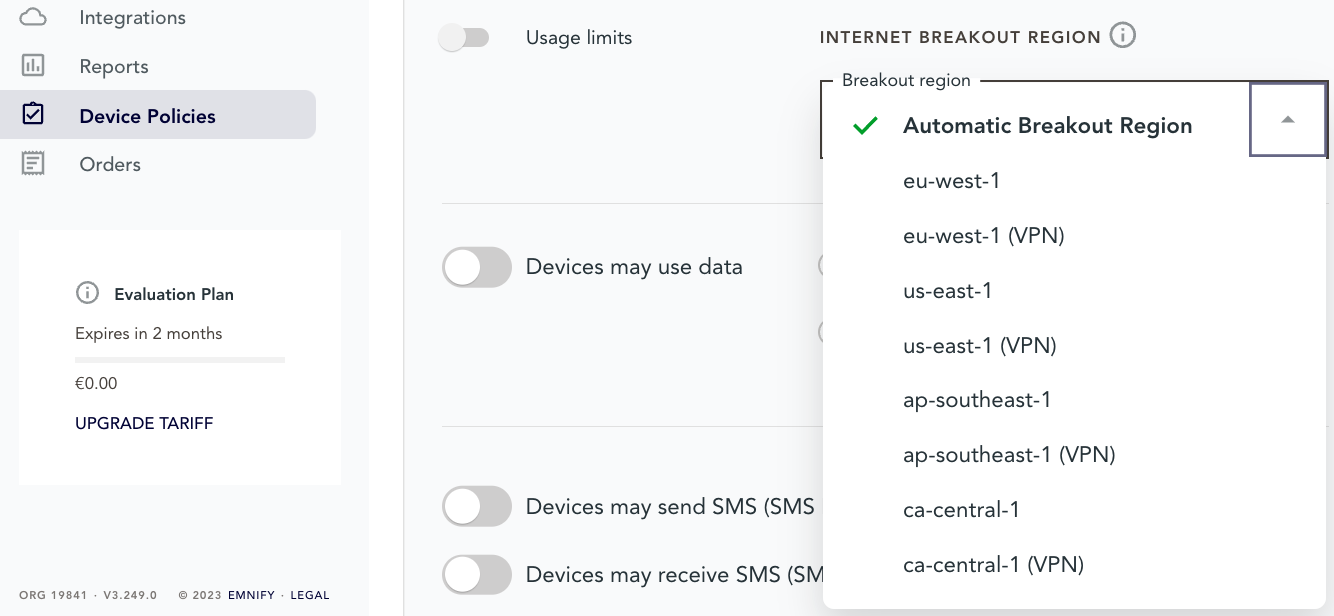
\includegraphics[width=15cm]{portal-device-policies-breakout-regions}
\end{center}

\pagebreak[4]

\section{emnify connectivity platform}

\begin{markdown}

emnify's connectivity platform provides solutions for configuring, deploying, maintaining and monitoring your IoT assets globally.
It it comprised of the following set of of tools.

## emnify Portal

\end{markdown}
The web-based \href{https://portal.emnify.com}{emnify Portal}\footnote{The emnify Portal is available via \href{https://portal.emnify.com}{https://portal.emnify.com}} is the Operation Center for the IoT SuperNetwork.

\begin{markdown}
The Portal allows Enterprise customers to monitor and manage all aspects of device communication -- from viewing real-time volume and costs, managing the SIM lifecycle and defining service policies to troubleshooting connectivity issues and executing and managing integrations. 
The web portal provides a fully responsive design, supporting Desktop, Mobile phones and Tablets.

### Operation Center

The emnify Portal serves as an operation center to monitor, manage and troubleshoot the device connectivity.

#### Dashboards
The Portal provides detailed reports about data and SMS traffic, costs for individual devices or the full organization, and in which networks the service has been used.

#### Device Details 
The portal provides an overview of all relevant information, such as real-time connection status, statistics, and detailed connectivity events which include location updates and PDP session creation logs for each device.

#### Device Policies
An Enterprise can define multiple service polices and coverage polices.
Devices can then be assigned to their respective policies thus creating groups which can simplify device management when large numbers of devices are deployed.
Each device group's access, traffic limits, and data plan only needs to be configured once for it to be applied to all devices in the group.

#### Location Information
Based on the location of the cell tower to which the device is connected, the emnify Portal displays map indicating the device's location.

### SIM management
\end{markdown}
\addspace
\begin{markdown}
- Ordering SIMs
- SIM lifecycle management
\end{markdown}
\addspace
\begin{markdown}
### User and Account Management
\end{markdown}
\addspace
\begin{markdown}
- Single-Sign On
- Multi-Factor Authentication
- User Roles
- Workspaces
\end{markdown}
\addspace
\begin{markdown}
## emnify APIs

### REST API

REST APIs are one way to integrate external services into your application.
The emnify API provides a variety of HTTP requests to integrate several emnify services into your application.

The emnify API is based on the OpenAPI Specification OAS3.

### GraphQL

GraphQL is a query language that enables you to define API call responses to match your use case and technical needs.

The emnify GraphQL API was initially developed internally to improve performance on the Portal.
In early 2023, we decided to release a preview version to customers.
We hope to collect feedback and continue adding features so that the functionality more closely matches our REST API.

### Data Streamer

With the emnify Data Streamer, enterprises can integrate real-time connectivity data directly into their third-party cloud services or business systems to build operational dashboards that visualize device, network, and application information side-by-side.
With this comprehensive view of their IoT solution and infrastructure connectivity data, they can quickly triage and resolve issues or create business reports.

### SDK

The emnify software development kits (SDKs) allow developers to manage their IoT devices using an intuitive set of APIs, including SIM state management and device connectivity operations.
emnify SDKs are currently available for Java and Python.

### No-Code

Zapier is a service that allows you to connect more than 4,000 applications -- including emnify -- to automate workflows.
With the available integrations you can automate device provisioning between emnify and your application.
For example, you can send configuration SMS to set the proper APN, when the device connects for the first time.
Other use cases are scheduled or application-triggered SIM activations/deactivations so that the SIM contract starts and ends with the device subscription of your customers.
The following events are available as triggers:
\end{markdown}
\addspace
\begin{markdown}
- All events in the Data Streamer
- Device enabled (SIM activated)
- Device disabled (SIM deactivated)
- Usage Limit Reached
\end{markdown}
\addspace
\begin{markdown}

The following actions are available:

\end{markdown}
\addspace
\begin{markdown}
- Send SMS to device
- Create a device (SIM configuration)
- Enable a device (SIM activation)
- Block current network (blacklist the last tried network)
\end{markdown}
\addspace
\begin{markdown}

Using the Zapier webhook, you can also use triggers from:

\end{markdown}
\addspace
\begin{markdown}
- SMS delivered notification
- Mobile originated (MO) SMS
\end{markdown}
\addspace
\begin{markdown}

### Events

The emnify system generates several types of events.
These events allow you to track notable system occurrences based on behavior.

Some common use cases for events on emnify include:

\end{markdown}
\addspace
\begin{markdown}
- **Triggers for custom business processes** (e.g., authentication or custom usage limitations configured on the [emnify Portal](usage#emnify-portal))
- **Monitoring** (e.g., SIM or data connection lifecycles)
- **Input for custom billing systems** (i.e., updating billing configuration, processing invoices, etc.)
\end{markdown}
\addspace
\begin{markdown}

Events are often used as triggers for custom business processes, for monitoring, and as input for custom billing systems.
They provide information about lifecycle transitions and configuration changes.

\end{markdown}
\pagebreak[4]
\section{Communication services}

\begin{markdown}

## Data

### Public internet breakout

An internet breakout is where data passes from a private network to the public internet.
For cellular networks the internet breakout is the home operator's central location -- the one that sold the SIM card.
This can pose a challenge for organizations with globally distributed devices.
Data might have to be routed through multiple countries or even across continents before arriving at the home operator's centralized data center before being sent to its final destination.

### Virtual Private Network

**Private APN**

A private Access Point Name (APN) is a solution that was developed to simply identify a gateway having specific policies for accessing a network that assigns static IP addresses to devices through which they can be remotely accessed.
The private APN was then used as an concentrated endpoint to help secure connectivity through policies like blocking public internet access.
Private APNs are often used in conjunction with a VPN.
However, emnify doesn't require a private APN for using a VPN.

**OpenVPN**

emnify's communication platform hosts an OpenVPN service that allows you to establish a private network between a device and any remote client location.
The remote client can be on the application server or any machine that wants to access the device remotely (such as operational staff).

Your IoT device doesn't need a private APN, OpenVPN software, or dynamic DNS resolution to use the OpenVPN service.
Through the emnify IoT eSIM, each device will have a static private IP address that you can use to identify and address the device.

At the same time, the IoT device can send data through the private tunnel to the IP address of the remote machine.

**Cloud Connect**

The data traffic of regular SIM cards is secured within the mobile network -- but traverses the public internet between the mobile network and the application, which makes the device and application susceptible to attacks and prohibits to easily establish a remote device session.

With emnify Cloud Connect your devices and application servers can communicate through a secure private network -- with a secure tunnel being established between the emnify platform and your cloud or on-premises application.

By eliminating the use of the public internet, Cloud Connect helps you better protect your application infrastructure against attacks like DDoS, port scanning while giving you the possibility to remotely access the devices.

### Inter-device communication

Traditionally, short message service center (SMSC) facilitates short message service (SMS) communications between devices on the network.
Text messaging and many Internet of Things applications depend on SMSCs to relay communications from one device to another.
In order to communicate with a network's SMSC, you'll need to enable your application to use Short Message Peer-to-Peer Protocol (SMPP).
This is a complex protocol that can be difficult to work with.

At emnify, we simplify SMS communication with our RESTful API.
This enables your devices to communicate over SMS using JavaScript Object Notation (JSON), and you don't have to worry about SMPP.

### Regional breakout

A regional internet breakout is when a distributed network routes data through regional data centers, typically through cloud service providers like Amazon AWS, Microsoft Azure, or Google Cloud.

emnify uses AWS to facilitate dynamic regional internet breakout to dynamically select the closest breakout region based on a device's location while using other availability zones as backups to prevent downtime.

## SMS

SMS messages can play a pivotal role in remote IoT device management and automation.
Since SMS works without a data connection, it's a reliable way to communicate with remote IoT devices.

By designing devices to accept SMS parameters, most manufacturers have eased the burden of configuring a fleet of devices, both for the initial connectivity configuration as well as for post-deployment configuration changes.

By leveraging SMS for specific tasks that would overwise require power-hungry data connections, devices can operate more efficiently by conserving battery power.

With SMS in place for your remote configuration, you can also use it to trigger additional actions on a device.
For example, if you wanted to perform an update, you could use SMS to trigger a firmware OTA update.

### SMS MO/MT

The ability to send and receive point-to-pont (P2P) SMS messages is often abbreviated as follows:

\end{markdown}
\addspace
\begin{markdown}
- **MO** Mobile-Originated, i.e., messages can originate (be sent) from this device
- **MT** Mobile-Terminated, i.e., messages can terminate (be received) at this device
\end{markdown}
\addspace
\begin{markdown}

### P2P SMS

Some countries implement a strict interpretation regarding what constitutes person-to-person (P2P) SMS communication.
In such cases, any application-mediated messaging is considered A2P instead, even if the originator and recipient are both non-commercial, individual consumers.

emnnify allows MO and MT SMS from external SMS devices.
Devices can be reached over the assigned MSISDN number from any regular mobile phone.

### A2P SMS

Application-to-Person (A2P) Short Message Service (SMS) refers to text messages sent from a software program to person or a SMS sent from a person to an application. Messages from an application are often automated and trigger based on a set of rules or conditions.
Messages to an application involve a request or command.

In the Internet of Things (IoT), end users and manufacturers rely on A2P SMS to do things like remotely set the Access Point Name (APN), reconfigure devices, "wake up" a device to go online, or send small measurement data to the application.

\end{markdown}

\begin{tcolorbox}[colback=blue!5!white,colframe=blue!75!black,title=Note]
\textbf{A2P and P2P Routing}\\
emnify distinguishes A2P SMS from P2P SMS based on the length of the source or the destination address.\\
If there are 8 digits or less (i.e., an invalid MSISDN), an SMS will be considered A2P.\\
If there are 9 digits or more, an SMS will be processed as MSISDN and will be considered P2P.\\
To dispatch SMS MO to your application and at the same time have P2P SMS enabled, the destination number must be limited to 8 digits or less.
\end{tcolorbox}


\begin{markdown}

**SMPP**

Short Message Peer-to-Peer Protocol (SMPP) is the system of rules that lets devices and software applications send and receive text messages over the internet.
Cellular Internet of Things (IoT) devices such as smart meters use the SMPP to transmit updates about resource consumption and location status.
When an event like a break-in or fire triggers a smart alarm system, it uses the SMPP to message the building owner, potentially with a link that allows them to access a camera feed.

**SMS via the emnify REST API**

If you're an IoT manufacturer, your device may rely on SMS communication.
In these cases, emnify can automate your SMS data exchange between device and application through the REST-API.
The REST-API does not only allow to programmatically send SMS to the device but also to retrieve the SMS data the device sends.

**SMS console in the emnify Portal**

The emnify Portal also provides an SMS console which allows an SMS to be sent to the device with a configurable source address.
In addition, the UI lists all SMSs that are received and sent by the device.

### SMS short codes

SMS short codes are often associated with automated services, each of which is assigned a unique short code and phone number.
Within the emnify core network, there is no SMS short code configuration required per specific customer or service.
All SMS messages that are sent and received from a specific customer will be forwarded through the API or SMPP.
This means each customer can use their own short codes and customize them based on their use cases.

\end{markdown}

\section{Network security services}

\begin{markdown}

Given the globally distributed nature of the devices, smaller footprints and lack of resources, it can get difficult to individually secure IoT devices.

emnify uses a SASE approach to simplify securing devices -- using several services specifically to protect customer data, filtering malicious content and preventing unauthorized access.

## SASE overview

Secure Access Service Edge ([SASE](/glossary#sase---secure-access-service-edge)) introduces a new architecture where networking and security functions are bundled in a cloud-delivered service.
You can apply the same security standards across all your devices independent of the location.
Moreover, you can integrate security features in your solutions right from the beginning.

Some of the features that [SASE](/glossary#sase---secure-access-service-edge) for IoT architecture includes are as follows:

\end{markdown}
\addspace
\begin{markdown}
- Dynamic Data Routing with Software-Defined Wide Area Network (SD-WAN)
emnify utilizes a SD-WAN to route data to the closest cloud region using the [Regional Breakout](iot-cloud-communication-platform#regional-breakout) concept.
In this way, latency and data stability is improved, and the end customer can be sure that data does not leave the continent and jurisdiction.
- Cloud Access Security Broker (CASB)
emnify allows centrally defining policies for the devices such as: networks that can be accessed, allowed IP addresses through which authorized users can remotely access devices.
All configuration is done in the central platform and applied wherever the device is.
\end{markdown}
\addspace
\begin{markdown}

## Virtual Private Network options

A Virtual Private Network (VPN) enables encrypted, targeted transmission of data over public networks such as the internet.
It establishes protected and self-contained networks with various devices.
A common use case is the connection of home offices or mobile employees.

### Private static IP

Assigning a device a private static IP address prevents computers or other devices outside the local network from directly connecting to it.

### Cloud Connect -- secure data transport

**AWS Transit Gateway**

Connect devices securely to AWS VPC without using public Internet.
Some of the features and benefits are:

\end{markdown}
\addspace
\begin{markdown}
- Devices and the application infrastructure reside within the same private network.
- Remotely access devices from AWS infrastructure via telnet / SSH.
- Device data does not traverse public internet.
- VPC / EC2 instances do not need public IP addresses.
- Fully scalable and managed AWS service.
\end{markdown}
\addspace
\begin{markdown}

**IPsec**

If your application is not on AWS but on any other cloud services or on-premise, you can utilize Cloud Connect for establishing an IPsec VPN connection.

With emnify you can set up an IPsec tunnel to securely transfer your data into your application server.

### OpenVPN -- remote access

OpenVPN is provided as a self-service for enterprise customers to get remote access to their devices from any OpenVPN client.
Customer VPN clients are authenticated with the credentials and application tokens of their emnify account to get remote access to devices.
OpenVPN establishes a single tunnel to the VPN gateways which are delivered in active-passive redundancy with automatic failover in case one VPN gateway becomes unavailable.

## Custom DNS

When a device establishes a connection, it uses a Domain Name Service (DNS) server to resolve a hostname to an IP address to which it can send data.
For example, a hostname such as `iot.example.com` will be mapped to an IP address like `192.0.2.1`.

Cellular providers typically provide a DNS service.
By default, emnify routes all DNS queries over Google's public DNS `8.8.8.8`.

For some devices and modules, it is possible to configure the DNS service.
For example, Quectel uses the `AT+QIDNSCFG` command, SIMcom `AT+CDNSCFG` command.
This is useful to be able to use your own or private DNS servers to secure and have better control over the solution.

Customers can also configure to use their own DNS, no matter if it is a public or a private one.
The DNS settings can be changed in the [emnify Portal](https://portal.emnify.com/) >> [**Device Policies**](https://portal.emnify.com/device-policies) >>  **New service policy** >>  **More options**

Utilizing a private DNS server which is not reachable via the public internet requires to set up a private network with the machine or a network where the private DNS server is located.
This can be done using Cloud Connect either with Amazon Transit Gateway or IPsec.
A tutorial on how to set up a DNS firewall based on a private DNS using Amazon Route 53 is available [here](https://www.emnify.com/en/developer-hub/dns-filtering).

## IMEI lock

For device manufacturers, SIM card theft is an issue because pluggable SIM cards can be removed from a device and then used to gain free internet access.
The [IMEI lock](/glossary#imei-lock)  feature prevents the use of SIM card in any other device by bounding the SIM to an IMEI.
The [IMEI](/glossary#imei---international-mobile-equipment-identity) is a unique device identifier.
When the automatic IMEI lock is configured, the emnify platform will bind the SIM cards to the first device that establishes a data connection.
All future device connections will only be allowed from this device.

## Centralized policies

Within the emnify platform, there is a separation between SIM card and the device, also referred to as "endpoint".
This allows you to configure policies on the device level rather than SIM level.
The device policies can be applied on a device group as well as at an individual level.

### Service policies

Service policies define which services are available for a group of devices. These policies include:

\end{markdown}
\addspace
\begin{markdown}
- Available radio access types (2G, 3G, 4G, NB-IoT)
- Monthly data and SMS limit
- SMS API configuration
- Custom DNS
- Breakout Region
- Available SMS service (MO/MT/P2P/A2P)
- Activation of Quota and Prepaid Management
\end{markdown}
\addspace
\begin{markdown}

### Coverage policies

Coverage policies define which tariff and network coverage is available for a group of devices.
This enables you to optimize the tariff based on the intended coverage.

The coverage policies include:

\end{markdown}
\addspace
\begin{markdown}
- The applied tariff for the group of devices
- The available networks organized in rate zones
\end{markdown}

\pagebreak[4]

\section{Support}

\begin{markdown}

emnify is dedicated to your success with our service.
We provide you with a choice of different plans, a globally-based customer success team, and support with global roaming to ensure that you have connectivity wherever you need it.

## Service Options

emnify offers a variety of support plans designed to ensure that your devices operate reliably in our network.
The **Standard** support plan is included for all customers at no additional cost.
It is the default service plan when registering through our website using the [emnify Portal](https://portal.emnify.com/).
For a detailed description of the standard services, please refer to our [Terms of Service](https://www.emnify.com/hubfs/20211001_terms_of_service_and_standard_service_level_obligations.pdf).

The **Business** and **Enterprise** plans offer premium customer service and can be bundled with your emnify subscription.
They are designed to reduce operational costs by detecting issues before they disrupt your business operations and by resolving [incidents](#incident-management) faster.

\end{markdown}
\begin{table}[H]
  \resizebox{\textwidth}{!}{%
  \begin{tabular}{|l|l|l|l|}
  \hline
  \textbf{Feature} & \textbf{Standard} & \textbf{Business} & \textbf{Enterprise} \\ \hline
  \textbf{Operating hours} & Mon-Fri 09:00-18:00 CET & 24x7x365 & 24x7x365 \\ \hline
  \textbf{Method of contact} & \begin{tabular}[c]{@{}l@{}}Tickets must be opened via webform.\\ Replies via email are possible.\end{tabular} & \begin{tabular}[c]{@{}l@{}}Tickets must be opened via webform.\\ Replies via email are possible.\end{tabular} & Webform, email, and phone \\ \hline
  \textbf{Help Center \& Knowledge Base} & Yes & Yes & Yes \\ \hline
  \textbf{Pre-scheduled event support} & Not included & Yes & Yes \\ \hline
  \textbf{Dedicated Support Agent} & Not included & Not included & Yes (EU-CET, US-EST or US-PST business hours) \\ \hline
  \textbf{Trace requests} & -- & \begin{tabular}[c]{@{}l@{}}1 simultaneous trace\\ Max 1 request/day\\ Max duration 24 hours/trace\end{tabular} & \begin{tabular}[c]{@{}l@{}}3 simultaneous traces\\ Max 1 request/day\\ Max duration 24 hours/trace\end{tabular} \\ \hline
  \textbf{\begin{tabular}[c]{@{}l@{}}Guaranteed response times:\\ • Critical incident\\ • Operational incident\\ • General issue / question\end{tabular}} & 7 business days & \begin{tabular}[c]{@{}l@{}}• 3 hours, 24x7x365\\ • 6 business hours\\ • 9 business hours\end{tabular} & \begin{tabular}[c]{@{}l@{}}• 1 hour, 24x7x365\\ • 3 hours, 24x7x365\\ • 6 business hours\end{tabular} \\ \hline
  \textbf{\begin{tabular}[c]{@{}l@{}}Target time to restore service: \\ • Critical incident\\ • Operational incident\end{tabular}} & -- & \begin{tabular}[c]{@{}l@{}}• 12 hours\\ • 10 business days\end{tabular} & \begin{tabular}[c]{@{}l@{}}• 4 hours\\ • 4 business days\end{tabular} \\ \hline
  \textbf{SLO} & \begin{tabular}[c]{@{}l@{}}Mobile Core: 98.5\%\\ Internet Breakout/VPN: 98.5\%\\ API/GUI: 98.5\%\end{tabular} & \begin{tabular}[c]{@{}l@{}}Mobile Core: 99.5\%\\ Internet Breakout/VPN: 99.5\%\\ API/GUI: 99.5\%\end{tabular} & \begin{tabular}[c]{@{}l@{}}Mobile Core: 99.95\%\\ Internet Breakout/VPN: 99.9\%\\ API/GUI: 99.5\%\end{tabular} \\ \hline
  \textbf{Root cause analysis} & Yes (Critical incidents) & Yes (Critical incidents) & Yes (Critical and operational incidents) \\ \hline
  \textbf{Length of service} & Monthly (automatic renewal) & Monthly (automatic renewal) & Minimum 12 months \\ \hline
  \end{tabular}%
  }
  \end{table}
\begin{markdown}

## Incident Management

emnify's network operation center (NOC) monitors the health of all cellular networks and services that emnify offers 24x7.
The NOC proactively identifies any degradation of service.
In case of an incident, it starts the incident management process that alerts a team of on-call engineers to start an investigation.

When an incident is triggered due to network-related events, the responding team will diagnose the fault and escalate the incident to emnify's carrier and roaming partners if necessary.
Optionally, any network causing a service disruption will be blocked so that devices can connect to alternate networks.

During an incident, emnify updates the [Status](https://status.emnify.com/) page for all services in order keep customers informed in real time about the status of the incident and its impact.

For critical and operational incidents, emnify conducts a root cause analysis (RCA) and issues a postmortem that provides details about the incident, which changes have been applied, and which measures are planned to guard against future incidents.

The incident management process is reviewed annually and certified by a third party as part of emnify's SOC2 audit.

## Roaming

Unlike typical mobile network operators ([MNO](https://www.emnify.com/iot-glossary/mno)s), emnify will also provide 24/7 support when your device is in roaming scenarios.
The emnify network operation center (NOC) has visibility of all networks in the world and can detect network service degradation. 
emnify will also investigate and follow up even when only your fleet of devices is affected.

Based on the direct and IoT/M2M specific roaming relationships with network operators, emnify has service-level agreements (SLAs) to resolve critical and operational incidents within specific timelines.

So you will never need to worry about roaming when your IoT devices are moved to another location, even if it is to another country or continent.
Support for the global deployment of IoT devices is a key feature of emnify's [Global IoT Network](/services/global-iot-network).

## Customer Success Manager

In addition to emnify's 24x7 support and network operation center (NOC), each customer has access to a Customer Success Manager (CSM).
CSMs comprise a globally distributed team with local working hours.
They are fluent in emnify's main supported languages: English, Spanish, Italian, French, and German.
The CSM team proactively engages with their customers to help them obtain value from the product and guide them through their journey.
They also conduct onboardings to get their customers acquainted with the platform and help with setting up integrations.

\end{markdown}

\end{document}  